% !TeX spellcheck = en_US

\chapter{Analytical Techniques for Plastic Debris in Soil}
\label{ch:analytical-techniques}

\paragraph{Abstract} Although most plastic pollution originates on land\marginnote{This chapter is based on: \fullcite{ThomasSample2020}.\par See \nameref{ch:author-contributions}, page~\pageref{ch:author-contributions}, for details.}, current research largely remains focused on aquatic ecosystems. Studies pioneering terrestrial research on plastic debris and microplastics have adapted analytical methods from aquatic research without acknowledging the complex nature of soil. Meanwhile, novel methods have been developed and further refined. However, methodical inconsistencies still challenge a comprehensive understanding of plastic occurrence and fate in and on soil. This chapter aims to disentangle the variety of state-of-the-art sample preparation techniques for heterogeneous solid matrices to identify and discuss best-practice methods for soil-focused polymer analyses. We show that soil sampling, homogenization, and aggregate dispersion are often neglected or incompletely documented. Plastic preconcentration is typically performed by separating inorganic soil constituents with high-density salt solutions. Not yet standardized but currently most used separation setups involve overflowing beakers to retrieve supernatant plastics, although closed-design separation funnels probably reduce the risk of contamination. Fenton reagent may be particularly useful to digest \ac{som} if suspected to interfere with subsequent quantification of plastic debris. A promising new approach is extraction of target polymers with organic solvents. However, insufficiently characterized soils still impede an informed decision on optimal sample preparation. Further research and method development thus requires thorough validation and quality control with well-characterized matrices to enable robust routine analyses for terrestrial plastic debris.

\section{Introduction}
\label{sec:analytical-techniques:intro}

A world without plastics seems difficult to imagine given the versatile possibilities for plastics use in all areas of our modern society. Since the advent of plastics mass production in the 1950s, plastics have found their way into everyday consumer products including packaging, mobility, building and construction, and agriculture \citep{GeyerProduction2017,KaweckiPolymerSpecific2019}. As a consequence, the global plastic production has increased exponentially from \SI{2}{\mega\tonne} in 1950 to \SI{359}{\mega\tonne} in 2018 \citep{PlasticsEuropePlastics2019,GeyerProduction2017}. The most produced polymers in terms of market shares are high- and low-density \ac{pe} (\SI{36}{\percent}), \ac{pp} (\SI{21}{\percent}), \ac{pvc} (\SI{12}{\percent}), \ac{pet} (\SI{10}{\percent}), \ac{pu} (\SI{8}{\percent}), and \ac{ps} (\SI{8}{\percent}) \citep{GeyerProduction2017}. Biodegradable plastics like \ac{pla} or \ac{pbat} have a combined market share of \SI{1.3}{\percent} \citep{BurgstallerStudy2018} but are gaining increasing attention as potential alternatives for conventional polymers.

Current estimates indicate that the extensive use of plastics has already piled up about \SI{5}{\giga\tonne} of plastic waste in the environment, which is equivalent to \SI{60}{\percent} of all plastic ever produced \citep{GeyerProduction2017}. \Citet{ThompsonPlastic2006} suggested that \SI{10}{\percent} of the produced plastic is entering the world's oceans leaving an unknown sink of \SI{50}{\percent}; that is \SI{2.5}{\giga\tonne}.
In line with this, plastic release into terrestrial systems has been hypothesized to be \numrange{4}{23} times higher than that into aquatic systems \citep{HortonLarge2017}. Accumulating plastic debris may adversely affect the soil structure and water dynamics \citep{deSouzaMachadoMicroplastics2019,deSouzaMachadoMicroplastics2020} as well as the fitness of soil biota including earthworms \citep{BootsEffects2019}, nematodes \citep{LeiPolystyrene2018}, and plants \citep{RilligMicroplastic2019,BuksWhat2020}. Nonetheless, only a few attempts have been made so far to better understand the extent of plastic pollution and fate in terrestrial ecosystems for an informed risk assessment. Soil, in particular, has been largely neglected as highlighted by \citet{HeMicroplastics2018}, who only found \SI{4}{\percent} of studies published on plastic debris actually focusing on soil. Consequently, terrestrial environments most likely play a key role in the world's plastic problem while remaining largely understudied.

Although scarcely quantified but regularly reviewed, plastics are assumed to enter the terrestrial environment via sewage sludge or biosolid application, use of agricultural plastic films, littering, and atmospheric deposition \citep[Chapter~\ref{ch:plastic-mulching};][]{HurleyFate2018,WangMicroplastics2019,BiancoAtmospheric2020}. While plastic items may be distributed and transported by air and water erosion \citep{BergmannWhite2019}, bioturbation \citep{HuertaLwangaIncorporation2017,RilligMicroplastic2017a}, or plowing \citep{vandenBergSewage2020}, they fragment into smaller debris due to physical abrasion, exposure to sunlight, or biological degradation \citep{BriassoulisAnalysis2015,CaiObservation2018}.
Plastic fragments are typically categorized by size into macroplastics (\SI{>5}{\milli\meter}), large microplastics (\SIrange{1}{5}{\milli\meter}), microplastics (\SI{1}{\micro\meter} to \SI{1}{\milli\meter}), and nanoplastics (\SI{<=1}{\micro\meter}) \citep{BraunMicroplastics2018,HartmannAre2019}. In addition, primary and secondary plastic can be distinguished in terms of particles being produced as such or resulting from fragmentation, respectively.
Further classification criteria address the particles' shape, chemical constitution, and material properties \citep{HartmannAre2019}. However, the scientific community has not yet established a consensual definition of polymeric properties despite the urgent need for a unified terminology defining criteria on the size, shape, color, and origin of plastics to facilitate the communication and comparability of data \citep{HartmannAre2019}.

The lack of harmonization is moreover immanent in the plethora of current approaches for plastic analysis of soil samples. Whereas \citet{BlasingPlastics2018} still concluded that plastic pollution in soil remained virtually unknown due to utterly lacking analytics, most recent reviews \citep{MollerFinding2020,Dioses-SalinasMethodological2020} outdo each other with new methods and microplastic findings. However, the majority of reported methods was initially developed for aquatic samples and potentially underestimates the complex nature of soil matrix that keeps sample preparation and polymer analysis challenging.

Analyzing soil requires careful consideration of the soil profile, soil type, and soil constituents like soil solutes, silicates, (swellable) clay minerals, and \ac{som} in varying quantities, grain and aggregate sizes, and densities \citep{BlumeScheffer2016}.
\Ac{som} is a dynamic, highly heterogeneous mixture of plant- and animal-derived litter at various stages of decomposition. The labile \ac{som} fraction contains easily degradable molecules like peptides, lipids, and carbohydrates, whereas the more stable fraction consists of more complex, polymeric macromolecules \citep{BronickSoil2005}.
Some of these soil constituents are suspected or have already been reported to interfere with polymer analysis so that they need to be removed or at least reduced during sample preparation \citep[Chapter~\ref{ch:py-gc-ms-method};][]{LoderEnzymatic2017,FischerSimultaneous2017}. Inorganic fractions such as silicates or clay are often physically removed by density separation, while organic fractions are wetchemically oxidized\sidenote{See \citet{HeMicroplastics2018} for a general introduction to analytical methods for microplastics in soil.}.
Apart from their purification efficiency, the selected methods further need to preserve the polymer analytes, which becomes particularly relevant for the analysis of nanoplastics or biodegradable polymers\sidenote{See \citet{FojtCritical2020} for a recent review on biodegradable plastics in soil.}. For both, reliable and quantitative analytical tools are still to be developed \citep{WangPoor2018,WahlNanoplastic2021}.

Previous reviews gave an extensive overview of potential occurrences of plastic debris in terrestrial systems \citep{HurleyFate2018,ZhuOccurrence2019,Dioses-SalinasMethodological2020,WuMicroplastics2020,MeixnerMicroplastic2020} and reflected on the suitability of generic methods for soil plastic analysis \citep{BlasingPlastics2018,MollerFinding2020}.
Our review, in contrast, specifically aims at critically discussing and evaluating current sample preparation techniques for the microplastic analysis of soil. Since soil-specific sample preparation methods are still scarce, we also assessed methods for other solid matrices like sediment or suspended organic matter for their transferability to soil with particular emphasis on their potential applicability and robustness against matrix interferences from various soil constituents.

To this end, we searched Web of Science, CAS SciFinder, Scopus, and Google Scholar literature data bases for search terms including ``microplastic'' or ``plastic debris'' in conjunction with ``soil'', ``biosolid'', ``sediment'', or ``organic matter''. Based on these findings and supplemented with cross references, we selected 229~original research articles, 37~reviews, 15~books or book chapters, and 25~reports, theses, and guidelines for further evaluation.
The reviewed preparation steps included soil drying and sieving, dispersion of soil aggregates, density separation, \ac{som} removal, and extraction with organic solvents.
Further, we give a brief overview of suitable options for microplastic analysis after soil sample preparation. We conclude with suggestions for best-practice sample preparation techniques and innovative ideas promoting the development of novel, refined methods for a soil-focused microplastic analysis.

\section{From the Field to the Lab}
\label{sec:analytical-techniques:field-to-lab}

\subsection{Sampling Strategies}
\label{sec:analytical-techniques:sampling}

The selection of an adequate sampling strategy is the most crucial step in environmental analysis. The choice of the sampling approach is determined by the research question and involves considerations of the hypothesized analyte distribution in the field, potential sources, or site geomorphology. As recently reviewed by \citet{MollerFinding2020}, common soil sampling strategies in accordance with \citet{ISO18400-102Soil2017} are equally applicable to microplastics and include hotspot or suspect sampling, systematic grid or transect sampling \citep[as conducted by][]{PiehlIdentification2018}, stratified sampling, and random sampling \citep{CorradiniEvidence2019}. The sampling area and sampling procedures are to be documented with field notes and photographs.
Sampling depths should be defined a priori and reflect the soil profile and management practices like plowing \citep{SponagelBodenkundliche2005,ISO18400-102Soil2017}. For agricultural fields, for instance, the Federal Soil Protection and Contaminated Sites Ordinance of Germany stipulates a minimum sampling depth of \SI{30}{\centi\meter} \citep{BBodSchVFederal1999}. Yet, the majority of agricultural screening studies for microplastics have so far limited their sampling depth to the topmost \SI{5}{\centi\meter} \citep{LiuMicroplastic2018,PiehlIdentification2018}.

Sampling guidelines by the US Department of Agriculture \citep{SchoenebergerField2012} and the US Environmental Protection Agency \citep{USEPALSASD2020} further recommend taking control samples of the same soil type from an area nearby that is not affected by the contaminant of concern. While this may be challenging for microplastics that ubiquitously enter soil via atmospheric deposition \citep{BergmannWhite2019}, this would offer the advantage of quantifying microplastic background levels, controlling contamination potentially introduced during sampling, or better understanding matrix interferences.
The risk of contamination may be reduced by using sampling equipment and containers that are free of plastics \citep{PiehlIdentification2018,ScheurerMicroplastics2018}. Plastic sledgehammers or nitrile gloves should thus be avoided \citep{WitzigWhen2020}.

The number of samples per site depends on the spatial extent of the investigated area. In order to cover the spatial variation of an exemplary field with 0.05--1 ha, German legislation \citep{BBodSchVFederal1999} recommends subdividing each field into at least three subplots.
For each subplot, one composite sample consisting of \numrange{15}{50} subsamples \si{\per\hectare} should be drawn \citep{ISO18400-102Soil2017}. While composite sampling has already been adopted by numerous microplastic field studies to increase sample homogeneity and representativity \citep{RamosPolyethylene2015,HuertaLwangaField2017,ScheurerMicroplastics2018}, others took single samples only \citep{PiehlIdentification2018,LiuMicroplastic2018,CorradiniEvidence2019}.

Minimal, yet representative sample quantities are typically guided by the soil's largest grain size. In accordance with \citet{ISO17892-4Geotechnical2016,ISO18400-102Soil2017}, a sample quantity of at least \SI{500}{\gram} is required for a fine soil with particles sizes smaller than \SI{2}{\milli\meter}. This is in line with existing microplastic screening studies of agricultural and floodplain topsoils that involved sample quantities of \SI{300}{\gram} to several kilograms per plot \citep{ScheurerMicroplastics2018,LiuMicroplastic2018,PiehlIdentification2018}.
By contrast, \citet{HuertaLwangaField2017} only took \SI{50}{\gram} of garden soil for the investigation of plastic transfer along a terrestrial food web. Larger sample quantities are generally advisable in order to acknowledge the heterogeneous distribution of discrete microplastic particles in soil. However, sample quantities of several kilograms usually increase both the sampling and analytical effort.
Furthermore, removing large quantities of fertile agricultural soil for sampling purposes may be contrary to sustainability efforts and economic interests of farmers and land owners. Here, stochastic particle distribution models \citep{HammersleyStochastic1972} may help to find optimum, representative sample quantities for a given soil texture and the expected microplastic particle sizes and concentrations.

\subsection{Soil Characterization}
\label{sec:analytical-techniques:soil-characterization}

Methods for the determination of basic soil characteristics like soil texture, bulk density, aggregate stability, pH, redox potential, \ac{som} or organic and inorganic carbon contents, and cation exchange capacity are detailed in several guidelines, such as \citet{ISO11277Soil2020,ISO11272Soil2017,DINEN15935Sludge2020}. For microplastic analysis, knowledge of the \ac{som} content, carbonates, and soil texture is particularly relevant as these parameters may influence sample preparation and subsequent microplastic quantification. For example, \citet{CorradiniEvidence2019} related decreasing recovery rates after density separation to elevated \ac{som} contents.
In addition, microplastics were recovered at higher rates from sandy soils than from loess or clay \citep{ZhangSimple2018}.
However, both studies did not provide information on how soil parameters were obtained. In contrast to \citet{ZhangSimple2018}, \citet{ScheurerMicroplastics2018} found no correlation between the soil texture and microplastic concentration in floodplain soil, but it remained unresolved to what extent potential microplastic relocation processes in the field may have masked microplastic recovery after sample preparation. This suggests that the description of sampling sites and soil characteristics needs to be more comprehensive in order to facilitate interstudy comparisons and to identify additional, yet uninvestigated, factors like pH or ionic strength potentially affecting sample preparation.

\section{Sample Preparation}
\label{sec:analytical-techniques:sample-prep}

\subsection{(Freeze) Drying}
\label{sec:analytical-techniques:drying}

Drying soil prior to analysis is imperative to obtain a comparable, water-free reference for microplastic contents or particle numbers. Independent of the analyte, \citet{ISO11464Soil2006} recommends soil drying at \SI{40}{\degreeCelsius} until weight is constant. Yet, drying conditions and procedures for subsequent microplastic analysis are still contrasting. Whereas \citet{vandenBergSewage2020} adhered to \citet{ISO11464Soil2006} and dried the soil at \SI{40}{\degreeCelsius} for \SI{72}{\hour}, \citet{LiuMicroplastic2018} chose \SI{70}{\degreeCelsius} for \SI{24}{\hour}.
However, temperatures above \SI{40}{\degreeCelsius} may affect the polymers' physical and structural properties by glass transition, melting, or degradation. For instance, the glass transition temperatures of \ac{pbt}, \ac{pmma}, and \ac{pa} are \num{40}, \num{50}, and \SIrange{50}{75}{\degreeCelsius}, respectively \citep{BeylerThermal2002}. Natural rubber and ethylene-vinyl acetate may start melting at temperatures of \SIrange{30}{65}{\degreeCelsius} \citep{BeylerThermal2002}. Temperatures of about \SI{60}{\degreeCelsius} typically initiate degradation of biodegradable polymers like \ac{pla} and \ac{pbat} \citep{BurgstallerStudy2018}. This is why freeze drying has been recommended as a more gentle alternative \citep{EndersWhen2020}. On the one hand, freeze drying has been reported to break cell walls and soil aggregates and thereby facilitate further sample preparation \citep{EndersWhen2020}. On the other hand, temperatures below the glass transition temperature increase polymer brittleness.
Frost wedging may further fragment microplastic particles and release additional cellular organic matter. In addition, freeze drying is more time-consuming than oven or air drying and often constrained by the size of the freeze dryer.

\subsection{Homogenization, Sieving, and Sorting}
\label{sec:analytical-techniques:homogenization}

Prior to further sample processing, soil is recommended to be adequately homogenized manually or by using automatic sample dividers. Laboratory subsamples and retention samples should be at least 200 g \citep{ISO11464Soil2006}. After homogenization, \citet{ISO11464Soil2006} further specifies sieving to fine soil \SI{<=2}{\milli\meter} \citep{ZubrisSynthetic2005,ZhangSimple2018}.
All subsequent soil analyses are performed on fine soil, and analyte contents are based on fine soil as common reference for interstudy comparisons.
This contrasts the common definition of microplastics of \SIlist{<=1;<=5}{\milli\meter} \citep{HartmannAre2019,BraunMicroplastics2018}.
Accordingly, \citet{PiehlIdentification2018} sieved soils to \SIlist{1;5}{\milli\meter}. \Citet{LiuMicroplastic2018,HuangAgricultural2020,ZhouMicroplastics2020} included all fractions below \SI{5}{\milli\meter}. In such cases, large microplastics may cover smaller particles and lead to systematic underestimation during spectroscopic analysis. We
thus suggest sieving to \SIlist{1;2;5}{\milli\meter} in compliance with standard mesh sizes of commercially available test sieves. Use of a sieving cascade may reduce the work load. However, it is currently poorly understood how excessive sieving might enhance the fragmentation of particles, in particularly aged, biodegradable,
or freeze-dried plastics.

\subsection{Dispersion of Soil Aggregates}
\label{sec:analytical-techniques:dispersion}

As microplastics may be incorporated into soil aggregates and thus not be easily separable from other soil constituents \citep{ZhangSimple2018},
additional preparative steps are required to promote the disintegration of soil aggregates and dispersion of grains. Although specified by \citet{ISO11464Soil2006}, grinding of soil samples for subsequent microplastic analysis will increase particle fragmentation and may induce melting by frictional heat. A simple alternative is initial shaking of soil samples in a dispersion agent such as aqueous sodium hexametaphosphate solution \citep{Garces-OrdonezMarine2019,VermaireMicroplastic2017,ZhouMicroplastics2020}. Additionally,
ultrasonication has been applied to soils suspended in deionized water \citep{ZhangDistribution2018,ZhangSimple2018} or in a salt solution prior to density separation \citep{LiuMicroplastic2018}. However, adequate sonication levels strongly depend on the soil type, in particular on the aggregate stability \citep{CerliSeparation2012}, and progressive sonication may increase the amount of light-density \ac{som} potentially interfering with density separation. Moreover, it has not yet been systematically assessed if or to what extent chemical dispersion agents or ultrasonication may cause interferences or enhance microplastic fragmentation, respectively.
Further method development is thus needed to scrutinize potential adverse effects on microplastic analysis to transfer established methods from soil science to terrestrial microplastics research.

\subsection{Density Separation}
\label{sec:analytical-techniques:density-separation}

\paragraph{Separation Principle}

The most common technique to preconcentrate or isolate microplastics from soil is density separation. Density separation exploits the buoyancy of plastic particles in solutions with a higher density than that of plastics ($\rho$ = \SIrange{0.9}{1.6}{\gram\per\cubic\centi\meter}),
while the soil mineral fraction (for instance silica, $\rho >$ \SI{2.0}{\gram\per\cubic\centi\meter}) remains at the bottom \citep{EndersEvaluation2020,LiuAnalytical2020}. To date there is no standardized density separation procedure for microplastic extraction from soils. In principle, the soil sample is mixed with a density solution, and floating plastic particles are collected after a certain amount of time. However, studies vary greatly in terms of sample amounts, applied density solutions, and the technical setup.

\paragraph{Density Solutions}

Various density solutions have already been used for isolating microplastic from soil, including deionized water, \ch{NaCl}, \ch{NaBr},  \ch{NaI}, \ch{CaCl2}, \ch{ZnCl2},
and sodium heteropolytungstate solutions. Additionally, ethanol, potassium formate,
\ch{ZnBr2}, sodium tungstate dehydrate, and \ac{spt} solutions have been tested for sediments but not yet for soil
(Table~\ref{tab:density-solutions}). Apart from density solutions, the applied ratios of soil to density solution vary greatly between 1:2 \citep{ChenMixing2020} and 1:25 \citep{ZubrisSynthetic2005}.
While soil-to-solutions ratios are often determined by the sample size and technical setup, they may be decisive for microplastic recovery.
However, this has not yet been addressed.

\begin{table*}[t]
	\centering\footnotesize
	\caption{Density solutions for the separation of plastic debris from solid matrices.}\label{tab:density-solutions}
	\begin{tabulary}{1.0\textwidth}{LLLLLL}
			\toprule
			{Density Solution} & {Density [\si{\gram\per\cubic\centi\meter}]} & {Evaluated Polymer Type(s)} & {Sample Type} & {Remarks} & {Reference} \\
			\midrule
			Ethanol (\SI{96}{\percent}) & \num{0.8} & Light-density \acs{som} & Plant material & Flotation of light-density \acs{som}; no microplastic separation & \citet{HerreraNovel2018} \\
			Deionized water & \num{1.0} & \acs{pe}, \acs{pp} & Clay soil, loess, and sandy soil & Not suitable for high-density polymers & \citet{ZhangSimple2018} \\
			\ch{NaCl} & \num{1.2} & \acs{pe}, \acs{pp}, \acs{ps}, \acs{pa}, \acs{pc}, \acs{pmma}, \acs{abs} & Farmland soil, marine sediment & Not suitable for high-density polymers & \citet{LiuMicroplastic2018,NuelleNew2014} \\
			\ch{NaBr} & \numrange{1.4}{1.6} & \acs{pe}, \acs{pp}, \acs{ps}, \acs{pet}, \acs{pvc}, \acs{pa}, \acs{pmma} & Agricultural and floodplain soil, sediment &  & \citet{LiuMethod2019,QuinnValidation2017} \\
			\ch{CaCl2} & \numrange{1.3}{1.5} & \acs{pe}, \acs{pp}, \acs{ps}, \acs{pet}, \acs{pvc}, \acs{pc}, \acs{pa}, \acs{pu}, \acs{abs} & Organic-rich topsoil & \ch{Ca^{2+}} may cause flocculation of \acs{som} & \citet{ScheurerMicroplastics2018} \\
			Potassium formate & \numrange{1.5}{1.6} & \acs{pe}, \acs{pp}, \acs{ps}, \acs{pet} & Lakeshore sediments & No validation performed & \citet{XiongSources2018} \\
			\ch{ZnCl2} & \numrange{1.5}{1.7} & \acs{ps} & Biosolids, soil & Expensive\textsuperscript{\textdagger}, corrosive, and harmful to the environment, may alter microplastics and cause foaming & \citet{WangPoor2018} \\
			\ch{ZnBr2} & \num{1.7} & \acs{pe}, \acs{pp}, \acs{ps}, \acs{pet}, \acs{pvc}, \acs{pa} & Sediment & Expensive\textsuperscript{\textdagger}, corrosive, and harmful to the environment & \citet{QuinnValidation2017} \\
			\ch{NaI} & \numrange{1.6}{1.8} & \acs{pe}, \acs{pp}, \acs{ps}, \acs{pet}, \acs{pvc}, \acs{pa}, \acs{pu} & Agricultural soil, sediment & Expensive\textsuperscript{\textdagger}, harmful to the environment & \citet{ClaessensNew2013,QuinnValidation2017,NuelleNew2014,HuangAgricultural2020} \\
			\acs{spt} & \numrange{1.4}{1.8} & \acs{pe}, \acs{pet}, \acs{pvc}, \acs{pa} & (Beach) sediment & Expensive\textsuperscript{\textdagger} & \citet{EndersEvaluation2020,FrereInfluence2017} \\
			Sodium tungstate dihydrate & \num{1.4} & \acs{pe}, \acs{pp}, \acs{ps}, \acs{pet}, \acs{pvc}, \acs{pc}, \acs{pa}, \acs{pu}, \acs{pmma}, \acs{eva}  & Sediment & Expensive\textsuperscript{\textdagger} & \citet{FriasStandardised2018} \\
			\bottomrule
			\multicolumn{6}{p{.9\textwidth}}{\footnotesize \textsuperscript{\textdagger} \num{>100}~Euros \si{\per\kilo\gram} \citep{CampanalePractical2020}.}
	\end{tabulary}
\end{table*}

Deionized water ($\rho$ = \SI{1.0}{\gram\per\cubic\centi\meter})
and saturated \ch{NaCl} solution ($\rho$ = \SI{1.2}{\gram\per\cubic\centi\meter}) are suitable for separating low-density polymers like \ac{pe}, \ac{pp}, and \ac{ps} from soil mineral matrices, while being cheap,
easily available, and not harmful to the environment \citep{MasuraLaboratory2015,ZhangSimple2018,LiuMicroplastic2018,ZubrisSynthetic2005,RennerData2019}.
\citet{ScheurerMicroplastics2018} reasoned that
\ch{Na+} may further promote dispersion of soil aggregates,
which could increase the extraction efficiency. While low-density microplastics can be specifically targeted using deionized water or \ch{NaCl}
solution, the extraction of denser particles is not possible. This particularly applies to \ac{pet} ($\rho$ = \SIrange{1.3}{1.6}{\gram\per\cubic\centi\meter}) and \ac{pvc} ($\rho$ = \SIrange{1.1}{1.6}{\gram\per\cubic\centi\meter}) \citep{ScheurerMicroplastics2018,VanCauwenbergheMicroplastics2015}.

To this end, saturated \ch{CaCl2} solution
($\rho$ = \SIrange{1.3}{1.5}{\gram\per\cubic\centi\meter}) has been proposed due to its low cost (\num{<100}~Euros \si{\per\kilo\gram}) and environmental friendliness \citep{StolteMicroplastic2015,ScheurerMicroplastics2018}. However, some unidentified, most likely organic floccules were observed after separation from soil \citep{ScheurerMicroplastics2018}. The authors suggested that divalent
\ch{Ca^{2+}} caused flocculation of organic substances through ion bridging. Thus, \ch{CaCl2} solutions cannot be recommended for the separation of microplastic in \ac{som}-rich samples.

While \ch{NaBr} solutions ($\rho$ = \SIrange{1.4}{1.6}{\gram\per\cubic\centi\meter}) did not result in significant improvement of microplastic recoveries from sediment \citep{QuinnValidation2017}, \citet{LiuMethod2019} found that \ch{NaBr}
outperformed both \ch{NaCl} and \ch{CaCl2} at separating various plastic types, sizes, and shapes from a range of different soil samples.
One reason for this discrepancy was probably the difference in the adjusted densities between both studies: \citet{QuinnValidation2017} used \SI{1.4}{\gram\per\cubic\centi\meter},
whereas \citet{LiuMethod2019} prepared a \SI{1.6}{\gram\per\cubic\centi\meter} solution. This raises the often neglected question of how density solutions are prepared and how this affects extraction efficiencies, once more underlining the need for a uniform protocol for the preparation of density solutions.

Potassium formate solutions ($\rho$ = \SIrange{1.5}{1.6}{\gram\per\cubic\centi\meter}) were used for separating microplastics from sediments \citep{StockSampling2019,XiongSources2018} but have not been tested for soils so far.
With regards to its density, it is reasonable to expect incomplete recovery of higher-density polymers. Yet, its environmental friendliness \citep{ECHAPotassium2020} would make it a solution worth testing.

A comprehensive comparison of different density solutions in sediment revealed that recovery rates of various microplastic types generally increased with the density of the solutions \citep{QuinnValidation2017}. This trend was independent of the particle size and may therefore equally apply to soil. For denser polymers like \ac{pet}
or \ac{pvc}, current studies therefore recommend high-density salt solutions such as \ch{ZnCl2} ($\rho$ = \SIrange{1.5}{1.7}{\gram\per\cubic\centi\meter}) or \ch{NaI}
($\rho$ = \SIrange{1.6}{1.8}{\gram\per\cubic\centi\meter}) \citep{MahonMicroplastics2017,HortonLarge2017,ZhangSimple2018}.
With prices \num{>100}~Euros \si{\per\kilo\gram} \citep{CampanalePractical2020}, these salt solutions are
\numrange{4}{10}~times more expensive than \ch{NaCl} and both classified as environmentally harmful \citep{ECHASodium2020,ECHAZinc2020}. Moreover, \ch{ZnCl2} is corrosive and may thus degrade microplastics \citep{HeMicroplastics2018}. In addition, \citet{ZobkovEvaluation2017} observed strong foaming when applying
\ch{ZnCl2} solution to organic-rich sediments. Although the cause was not further investigated, excessive foaming may be problematic for restricted container volumes and pose difficulties for retrieving the supernatant. By contrast, \ch{NaI} solution may cause blackening of some filter papers, which may require an additional transfer step to a clean filter \citep{QuinnValidation2017}.

A promising solution is sodium heteropolytungstate ($\rho$
= \SI{1.5}{\gram\per\cubic\centi\meter}), which was successfully used for separating microfibers from soil and earthworm depurates \citep{Prendergast-MillerPolyesterderived2019}. Similar solutions, including sodium tungstate dihydrate ($\rho$ = \SI{1.4}{\gram\per\cubic\centi\meter}) \citep{FriasStandardised2018}, and \ac{spt}
($\rho$ = \SIrange{1.4}{1.8}{\gram\per\cubic\centi\meter}) \citep{BallentSources2016,EndersTracing2019,EndersWhen2020,CorcoranPlastics2009} were used for sediment samples but have not yet been applied to soil.
\Citet{EndersWhen2020} provided a detailed guidance protocol for an entire microplastic (\SI{10}{\micro\meter} to \SI{5}{\milli\meter}) extraction pipeline with \ac{spt}
solution as separation agent. Nevertheless, \ac{spt} is costly (\num{>100}~Euros \si{\per\kilo\gram}) \citep{CampanalePractical2020}, and a systematic validation including recovery tests for soil samples is still missing. This impedes comparing the general performance of \ac{spt}
with more commonly used salt solutions.

In order to maximize separation efficiency and reduce the consumption of higher-density solutions, multiple-step separation procedures have been introduced either by using the same solution several times \citep{LiuMicroplastic2018,HuangAgricultural2020} or by applying lower- and high-density solutions sequentially \citep{NuelleNew2014,HurleyValidation2018,CorradiniEvidence2019,vandenBergSewage2020,DekiffOccurrence2014,ZhouDistribution2018}. Typically, deionized water \citep{vandenBergSewage2020,HurleyValidation2018} or \ch{NaCl} solution \citep{NuelleNew2014,DekiffOccurrence2014,ZhouDistribution2018,FrereInfluence2017} are used first. In a second step, residues may be subjected to \ch{NaI} solution to extract high-density polymers. \Citet{FrereInfluence2017} chose sodium tungstate for sediment samples instead and completely recovered \ac{pet},
\ac{pvc}, and \ac{pa} particles (\SI{5}{\milli\meter}). \Citet{CorradiniEvidence2019} even performed a three-step density separation for sewage sludge and soil samples with deionized water, \ch{NaCl}, and \ch{ZnCl2} solution, which increased recovery for all plastics examined, but most significantly for
\ac{pvc}. However, recovery rates were not provided in detail.

Although not examined so far, low-density solutions may be equally valuable for reducing \ac{som} ($\rho <$ \SI{1.6}{\gram\per\cubic\centi\meter}) \citep{CerliSeparation2012} in the soil matrix without altering polymers. For example, ethanol (\SI{96}{\percent}, $\rho$ = \SI{0.8}{\gram\per\cubic\centi\meter}) has been suggested for separating plastics from less dense biological material \citep{HerreraNovel2018}. While such an intermediate treatment step may facilitate and reduce material consumption for further sample preparation, the risk of losing light-density plastics needs to be carefully evaluated. When deciding on several density separation steps, potential tradeoffs between improved separation efficiency and increased risks of contamination or loss of microplastics need to be taken into account.

In general, density solutions have proven their suitability for separating microplastics from the soil matrix. Solutions with higher densities like \ch{NaBr}, \ch{NaI}, \ch{ZnCl2}, or \ac{spt} ($\rho$ =
\SIrange{1.6}{1.8}{\gram\per\cubic\centi\meter}) extract a wide range of polymers at the expense of potentially co-extracting \ac{som} ($\rho <$
\SI{1.6}{\gram\per\cubic\centi\meter}) \citep{CerliSeparation2012} and thus require additional purification. By contrast, lower-density solutions (deionized water, \ch{NaCl}; $\rho$ = \SIrange{1.0}{1.2}{\gram\per\cubic\centi\meter}) may be preferred when targeting specific polymers or for reducing costs, operational effort, or environmental impact. Therefore, the suitability of a specific solution needs to be assessed on a case-by-case basis in accordance with the research question, the soil composition, and polymers of interest.

\paragraph{Recycling of Salt Solutions}

According to the principles of green chemistry, the quantity,
hazardousness, and disposal of chemicals should be reduced as much as possible \citep{AnastasGreen2009}. Thus, recycling is imperative
for expensive solutions and solutions of environmental concern used for density separation. Several recycling attempts have already been described for \ch{NaBr}, \ch{NaI}, \ch{ZnCl2}, potassium formate, and \ac{spt}. \Citet{KedzierskiEfficient2017} showed that \ch{NaI} solutions used for density separation of sediments can be recycled up to ten times by evaporation without decreasing the separation efficiency. Another approach evaluated \ch{ZnCl2} recycling via membrane filtering (\SI{0.45}{\micro\meter}) \citep{RodriguesImproving2020}. Over five filtration cycles,
microplastic recovery remained above \SI{95}{\percent}. Potential changes in density or pH were not reported. \Citet{StockSampling2019} recycled potassium formate by filtering, however, without assessing recoveries. \Citet{LiuMethod2019} constructed an automatic flow system that allowed for immediate recycling and continuous use of density solution.
This substantially reduced the needed amount of \ch{NaBr} solution and recovery rates remained \SI{>90}{\percent}. Recycled solutions may be stored either as solution \citep{LiuMethod2019,RodriguesImproving2020} or as extracted salt \citep{KedzierskiEfficient2017}. Although most authors reported cost and material reductions, it remains important to note that recycling and storage require additional working time, materials, space, and energy.

\paragraph{Instrumental Setups}

The simplest technique for density separation is direct mixing of sample and solution by manual shaking or stirring and subsequent settling in an appropriate sample container \citep{MahonMicroplastics2017,DekiffOccurrence2014,ZhangSimple2018,LiuMethod2019}. However, automated and controlled shaking in overhead \citep{QuinnValidation2017} or platform systems \citep{vandenBergSewage2020}, magnetic \citep{HuangAgricultural2020} or electric stirring \citep{ImhofNovel2012} may be preferred to increase reproducibility and method standardization.

Containers used for density separation vary greatly, ranging from beakers and separation funnels to more complex setups. Glass beakers are used most widely \citep{QuinnValidation2017,KleinOccurrence2015,LiuMicroplastic2018,ZobkovEvaluation2017,HuangAgricultural2020,ZhouMicroplastics2020}, followed by bottles \citep{HurleyValidation2018},
Erlenmeyer flasks \citep{WangPoor2018}, and centrifuge tubes \citep{CorradiniEvidence2019}. In some studies, separation devices were self-built \citep{ImhofNovel2012,RennerData2019}. Depending on the container of choice, a \SI{5}{\gram}
\citep{CorradiniEvidence2019} to up to \SI{6}{\kilo\gram} \citep{ImhofNovel2012} sample can be processed, requiring \SI{20}{\milli\liter} to \SI{12}{\liter} density separation solution,
respectively. Although rarely specified, the height of the container may be important as it determines the distance between the denser and lighter fraction and thereby the separation efficiency \citep{MahatSeparation2017}. Furthermore, container materials should be free of plastics to avoid contamination or sticking of plastic particles to the inner surface of the container.

To further promote separation, \citet{EndersWhen2020} designed a spiral conveyor rotating inside a separation funnel to constantly transport the sample upwards. Thereby, the sample disperses more efficiently, which facilitates microplastic separation from the heavier soil matrix. \Citet{NuelleNew2014} proposed an air-induced overflow system,
exposing the sample to turbulences by continuous air-bubbling potentially benefiting the separation of lighter particles from denser matrix. The method was efficient at reducing the amount of sediment for further treatment steps. A more advanced setup was developed by \citet{RennerData2019} using larger air bubbles for dispersion and finer ones as adhesive surfaces for separating microplastics from the matrix. The setup also minimized dead spaces to ensure that no plastic particles would be retained in the container. The method seems promising as \SI{>90}{\percent} of microplastic spikes were recovered from sand samples within 20 min. Although the authors propose its suitability for soil samples, an evaluation is still pending. Notably,
when \citet{ScheurerMicroplastics2018} combined stirring with continuous air-bubbling for soil samples, the method did not result in a significantly higher extraction efficiency. One possible challenge for the applicability of air bubbling systems to soil is that very fine textured, clayey soils or soils with very dense minerals may form a sludge at the bottom of the vessel, blocking the air inlet. Instead, \citet{ScheurerMicroplastics2018} used centrifugation to reduce the processing time. While others also centrifuged soil samples in density solutions \citep{vandenBergSewage2020,CorradiniEvidence2019}, only \citet{ScheurerMicroplastics2018} reported recoveries (\SI{>=93}{\percent}).

In general, separation protocols vary not only in terms of the density separation procedure but also in treatment times (\SI{10}{\second} to \SI{2}{\hour}) \citep{NuelleNew2014,vandenBergSewage2020} and settling times (\SI{5}{\minute} to \SI{24}{\hour}) \citep{HanOptimized2019,ScheurerMicroplastics2018}. For adjusting these procedural parameters, plastic and soil mineral particle sizes as well as the \ac{som}
content and soil aggregate stability may provide a reference to evaluate suitable settling times \citep{WangPoor2018}.

\paragraph{Sample Collection}

After the separation procedure, microplastics floating on the solution surface need to be collected and isolated for further treatment and analysis. A simple and low-cost approach is to collect microplastics by decanting \citep{BesleyStandardized2017,HuangAgricultural2020,ZhangSimple2018,ScheurerMicroplastics2018}. Since microplastics have the tendency to adhere to the inside of container walls \citep{NakajimaSmall2019}, repeated density separations may be necessary to ensure the complete transfer of all microplastics. However, this results in prolonged processing times and increases the risk of contamination. Floating \ac{som} is particularly challenging for the decanting method.

Microplastics can also be further retrieved by suction. First applications involved pipettes to collect synthetic fibres from sludge and soil \citep{ZubrisSynthetic2005,Prendergast-MillerPolyesterderived2019}. \Citet{ScheurerMicroplastics2018} used a vacuum pump to aspirate the topmost layer of the density solution with the microplastics and transferred them to a second vessel for collection.
The inherent risk is that particles floating directly on the surface are not collected and are lost for analysis as tubes need to be submerged for vacuum pumping. Rinsing of tubes may also increase the demand of solution media. Adding surfactants such as polysorbate~80
\citep{EndersWhen2020} may reduce adhesion to separation equipment.
However, this has not been tested for soil so far.

Most of the recently developed systems are based on overflow of the supernatant through the continuous addition of density solution \citep{NuelleNew2014,ZhouMicroplastics2020,VermeirenMicroplastic2020,WangPoor2018,LiuMicroplastic2018,LiuMethod2019,HanOptimized2019}. With this, microplastics may adhere not only to inner but also to the outer container walls, which complicates particle collection. Moreover, such open constructions are extremely prone to contamination.

By contrast, separation funnels\sidenote{See \citet{EndersWhen2020} for illustrations.} have an outlet at the bottom of the apparatus that is used to drain the settled mineral fraction before collecting the supernatant \citep{WangPoor2018,NuelleNew2014,MahonMicroplastics2017}. Separation funnels are prone to clogging if the outlet is too narrow. This particularly applies to very fine or very coarse soil. Clogging may be mitigated by either adjusting the diameter of the outlet valves \citep{EndersWhen2020} or carefully stirring up the sediment. However, the latter would favor particle adhesion to stirrers and might cause the resuspension of fine soil. Nevertheless, separation funnels offer the advantage of using a single container, which reduces dead spaces as well as the risk of contamination and analyte loss.

To further facilitate sample collection, density separation apparatuses were customized in such a way that a bottom chamber containing the dense material can be physically separated from a top chamber with the extracted microplastics, for instance, by use of a ball valve \citep{ImhofNovel2012,ZobkovEvaluation2017,CoppockSmallscale2017,MahatSeparation2017}.
Depending on the chamber geometry and the type of ball valve, dead spaces may retain microplastics leading to reduced recoveries. Furthermore, fine clay particles may block the valve after long-term use.

Finally, microplastics are typically collected on membrane filters for subsequent analysis. Depending on the target particle size and analytical approach, decisions need to be made regarding the filter mesh width and material \citep{MintenigIdentification2017,LoderFocal2015}. A first systematic evaluation of different filter materials was conducted by \citet{LoderFocal2015} who found \ch{Al} oxide and \ac{pc} filters the least interfering with identification via \ac{ftir} spectroscopy. However, using filters made from plastic, such as
\ac{pc} \citep{LoderFocal2015} or nylon \citep{LiuMicroplastic2018}, may exclude these polymers from further analysis. While glass fiber filters come in as being useful for particle collection \citep{HuangAgricultural2020,ChenMixing2020}, they were reported unsuitable for spectroscopic methods \citep{LoderFocal2015}. Cellulose-based filters may be chosen instead \citep{ZhouMicroplastics2020,CorradiniEvidence2019,vandenBergSewage2020}, but interactions with density solutions may alter filter properties \citep{QuinnValidation2017}. Thus, potential interferences of altered filter material during analysis need to be tested. Although not always specifically stated, the filter mesh size determines the lower size limit for plastic detection. Reported mesh widths are often larger than \SI{5}{\micro\meter} \citep{HuangAgricultural2020,ZhouMicroplastics2020}. Consequently, the usage of filters for sample collection implies a systematic loss of the smallest microplastic fraction (\SI{<=5}{\micro\meter}), and the complete nanoplastic fraction (\SI{<1}{\micro\meter}). This is particularly relevant for thermoanalytical methods, which are theoretically capable of capturing these fractions. Moreover, there is a potential tradeoff between minimizing mesh sizes and the filtration capacity, especially for soils high in light-density \ac{som} where filters may easily get clogged.

\subsection{\Acs{som} Removal}
\label{sec:analytical-techniques:som-removal}

With $\rho <$ \SI{1.6}{\gram\per\cubic\centi\meter} \citep{CerliSeparation2012} the density of \ac{som} is similar to that of microplastics ($\rho$ = \SIrange{0.9}{1.6}{\gram\per\cubic\centi\meter}) \citep{EndersEvaluation2020} and can thus be only partially removed by density separation. \Ac{som} removal is important as
\ac{som} constituents may interfere with subsequent microplastic analysis. Four groups of digestion agents for organic matter removal can be distinguished:
\begin{enumerate*}
	\item alkaline \ch{KOH}	or \ch{NaOH} solutions,
	\item acids including \ch{HNO3} and \ch{H2SO4},
	\item oxidants like \ch{H2O2} or Fenton reagent, and
	\item enzymes, for example proteinase~K
\end{enumerate*}
(Table~\ref{tab:som-removal}) \citep{DehautMicroplastics2016}.
Different digestion agents may be applied sequentially to optimize removal efficiencies.

\begin{table*}
	\centering\footnotesize
	\caption{Suitability of digestion agents for the removal of \ac{som} for microplastic analysis.}\label{tab:som-removal}
	\setfloatalignment{t}
	\begin{tabulary}{1.0\textwidth}{LLLLLLLL}
		\toprule
		{Reagent} & {Sample Type} & {Evaluated Polymers} & {Extraction Time [\si{\day}]} & {Temp. [\si{\degreeCelsius}]} & {\Acs{som} Removal Efficiency [\si{\percent}]} & {Deteriorated Polymers} & {Reference} \\
		\midrule
		\ch{KOH} & Loamy sand & \acs{pe}, \acs{pp}, \acs{ps}, \acs{pet}, \acs{pa}, \acs{pc}, \acs{pmma}  & \num{1} & \num{60} & \num{30(20)} & \acs{pc} & \citet{HurleyValidation2018} \\
		\ch{NaOH} & Loamy sand & \acs{pe}, \acs{pp}, \acs{ps}, \acs{pet}, \acs{pa}, \acs{pc}, \acs{pmma} & \num{1} & \num{60} & \num{70(20)} (\SI{1}{\Molar}), \num{60(40)} (\SI{10}{\Molar}) & \acs{pet}, \acs{pc} & \citet{HurleyValidation2018} \\
		\ch{HNO3} & Floodplain soil & \acs{pe}, \acs{pp}, \acs{ps}, \acs{pet}, \acs{pvc}, \acs{pa}, \acs{pc}, \acs{pu}, \acs{abs} & \num{2} & \num{90} & Higher than \ch{NaOH}, \ch{H2SO4}, \ch{H2O2} & \acs{abs}, \acs{pa}, \acs{pet} & \citet{ScheurerMicroplastics2018} \\
		\ch{H2SO4} & Floodplain soil & \acs{pe}, \acs{pp}, \acs{ps}, \acs{pet}, \acs{pvc}, \acs{pa}, \acs{pc}, \acs{pu}, \acs{abs} & \numlist{1;4;7} & \num{90} & Lower than with \ch{HNO3} & Not tested & \citet{ScheurerMicroplastics2018} \\
		\ch{H2O2} & Loamy sand & \acs{pe}, \acs{pp}, \acs{ps}, \acs{pet}, \acs{pa}, \acs{pc}, \acs{pmma} & \num{1} & \num{60} & \num{100(10)} & \acs{ps} & \citet{HurleyValidation2018} \\
		\ch{H2O2} & Agricultural soil & \acs{pe}, \acs{pp}, \acs{ps}, \acs{pet}, \acs{pvc}, \acs{pa}, \acs{pc}, \acs{pmma}, \acs{abs}  & \num{1} & \num{60} & Not reported & Not reported & \citet{LiuMethod2019} \\
		\ch{H2O2} & Sediment & \acs{pe}, \acs{pp}, \acs{ps}, \acs{pet}, \acs{pvc}, \acs{pa}, \acs{pc}, \acs{pu}, \acs{abs} & \num{7} & RT & Not reported & \acs{pet}, \acs{pvc},\acs{pc}, \acs{pa}, \acs{pu}R, \acs{pp}, \acs{pe} & \citet{NuelleNew2014} \\
		\ch{H2O2} & Loamy sand & \acs{ps}, \acs{pp}, \acs{pe}, \acs{pet}, \acs{pa}, \acs{pc}, \acs{pmma} & \num{1} & \num{70} & \num{100(10)} & \acs{pa}, \acs{ps} & \citet{HurleyValidation2018}  \\
		Fenton reagent & Loamy sand & \acs{pe}, \acs{pp}, \acs{ps}, \acs{pet}, \acs{pa}, \acs{pc}, \acs{pmma} & \num{1} & \num{40} & \num{100(10)} & None & \citet{HurleyValidation2018} \\
		\bottomrule
		~
	\end{tabulary}
\end{table*}

Alkaline solutions are typically used for denaturation of proteins in biota. When applied to a floodplain loamy sand containing \SI{5.8}{\percent} \ac{som},
however, NaOH (\SIlist{1;10}{\Molar}) and KOH (\SI{1.8}{\Molar}) solutions only removed
\SIrange{35}{68}{\percent} \ac{som} \citep{HurleyValidation2018}. The researchers suggested that humins and alkali-insoluble compounds could not be degraded and removed from the sample. In addition, \ch{NaOH} resulted in a severe \ac{pet} and \ac{pc} mass loss of up to \SI{30}{\percent}, while \ch{KOH} partially degraded \ac{pc}. Alkaline treatments may even more severely affect biodegradable plastics. \Citet{KuhnUse2017},
for instance, reported complete loss of \iac{pla} bag after purification with \SI{1}{\Molar} \ch{KOH}.

Similarly, \ch{HCl} and \ch{HNO3} have been discussed as potential digestion agents for \ac{som} \citep{BlasingPlastics2018}. Concentrated
\ch{HNO3} (\SI{65}{\percent}) completely removed \ac{som} (\SI{>30}{\percent})
from a floodplain soil whereas \SI{96}{\percent}
\ch{H2SO4} and \SI{13}{\percent} potassium hypochlorite left \SIlist{3;6}{\percent} of organic residues,
respectively \citep{ScheurerMicroplastics2018}. However, \ac{abs}, \ac{pa}, and \ac{pet} were partly degraded or fragmented into smaller particles \citep{ScheurerMicroplastics2018}.

The majority of studies addressing the removal of \ac{som} used \ch{H2O2} for sample preparation
(Table~\ref{tab:som-removal}). This may be attributed to the fact that \ch{H2O2} has been successfully applied to sediments in previous studies \citep{NuelleNew2014,ImhofNovel2012}. In line with this, \citet{HurleyValidation2018}
removed \SIrange{96}{108}{\percent} \ac{som} from a loamy sand with \SI{30}{\percent}
\ch{H2O2} at \SI{70}{\degreeCelsius}. However, \ac{pa} particles were destroyed and \ac{ps} particles partly degraded. Experiments at room temperature revealed changes in color and size for \ac{pe}, \ac{pp}, \ac{pet}, \ac{pvc},
\ac{pc}, \ac{pa}, and \ac{pu} after \SI{7}{\day} \citep{NuelleNew2014}. While effective for removing vegetal litter, degrading effects on microplastics were also mentioned for a three-stage method developed by \citet{DuanDevelopment2020}.
Therein, \ch{H2O2} (\SI{30}{\percent}) was consecutively added at temperatures of \SIlist{70;100}{\degreeCelsius} and left for digestion for \SIrange{1}{7}{\hour}. With regards to previous findings \citep{HurleyValidation2018}, polymer degradation was probably related to the elevated reaction temperatures. Thus, temperature and time should be carefully adjusted in order to preserve the polymer analytes. In addition, the \ac{som} removal efficiency most likely depends on the composition of the examined soil. \ox{3,Fe} and \ch{Mn} (sesqui)oxides, for instance,
were indicated to catalyze the disproportionation of
\ch{H2O2} into water and oxygen before an oxidation reaction was initiated \citep{PetigaraMechanisms2002}. Interactions with clay minerals, carbonate coatings, or occlusion in soil aggregates may further protect \ac{som} from oxidation \citep{MikuttaOrganic2005}, which calls for more potent and selective \ac{som} removal agents.

Fenton reagent, an acidified solution (pH \numrange{3}{5}) of \ch{H2O2} and a \ch{Fe^{2+}} catalyst, produces hydroxyl and hydroperoxyl radicals at high yields.
Hydroxyl radicals are particularly effective in degrading \ac{som} (\SI{100(10)}{\percent} removal efficiency) already at room temperature. Additional cooling (\SI{<=40}{\degreeCelsius}) is advisable since the reaction is extremely exothermic \citep{HurleyValidation2018}.
In contrast to treatments with \ch{H2O2} at elevated temperature, \citet{HurleyValidation2018} did not observe any detrimental effect on polymer sizes and masses after Fenton digestion, which may be attributed to the lower reaction temperatures (\SI{<=40}{\degreeCelsius}). This may further explain why \citet{VermeirenMicroplastic2020} only recovered \SI{90}{\percent} \ac{pe} after Fenton digestion of organic-rich sediments without monitoring the reaction temperature. Although promising, Fenton digestion has not yet been widely applied for soil sample preparations, but it should be further pursued.

Enzymatic digestion makes use of a variety of different enzymes for the selective degradation of potentially interfering matrix constituents without altering polymer analytes \citep{LiuAnalytical2020}. These enzymes include proteinase~K \citep{ColeIsolation2014}, trypsin \citep{Courtene-JonesOptimisation2017},
lipase and amylase \citep{RailoApplication2018}, corolase \citep{LaversDetection2019},
protease, cellulase, and chitinase \citep{LoderEnzymatic2017}. So far, no protocol on the enzymatic purification of soil samples for microplastic analysis has been published. Only a Swedish report by Sweden Water Research \citep{LjungMicroplastics2018} lists commercial cellulase, esterase,
and xylanases as enzymes potentially suitable for soil sample preparation,
however, without reporting removal efficiencies or recovery rates.
Enzymes targeting specific \ac{som} constituents therefore still need to be investigated. However, even the enzymatic digestion of wastewater samples is often incomplete so that several enzymes need to be applied successively and in conjunction with oxidative treatments \citep{LoderEnzymatic2017,MintenigIdentification2017}. Such multi-step protocols may be costly and easily take more than two weeks per sample \citep{LoderEnzymatic2017}.
Furthermore, long and complicated sample preparation methods probably increase the risk of contamination, for instance, during additional filtering steps.

In terms of removal efficiencies and microplastic recoveries, oxidizing agents like Fenton reagent and \ch{H2O2}
are currently considered the most suitable for \ac{som} removal. However,
biodegradable plastics and nanoplastics are still largely understudied and will require a reevaluation of sample preparation methods to avoid systematic underestimations. It is still not fully understood to what extent soil constituents like \ch{Mn} oxides or clay minerals may interfere with oxidative techniques. Since most studies investigated agricultural soils, it is unclear if current methods are readily transferable to soils with a different \ac{som} composition like chernozems or kastanozems. A thorough soil characterization, and thereby a better understanding of potential matrix interferences, may help the advancement of soil-specific sample preparation methods.

\subsection{Extraction with Organic	Solvents}
\label{sec:analytical-techniques:solvent-extraction}

In addition to density separation and \ac{som} digestion, the use of organic solvents for the extraction of microplastics from solid matrices has gained growing attention within the scientific community
(Table~\ref{tab:extraction-methods}). \Citet{FabbriAnalysis2000} first extracted \SI{1}{\gram\per\kilo\gram} \ac{pvc} and \ac{ps} debris from beach sand with \ac{dcm} using a Soxhlet apparatus.
\Ac{pvc} recovery was \SI{85}{\percent} while \ac{ps} was evaluated qualitatively. In recent years, further technical and analytical developments have lowered recoverable concentrations by a factor of 20--50 \citep[Chapter~\ref{ch:py-gc-ms-method};][]{PeezQuantitative2019,DierkesQuantification2019} and made a broader spectrum of polymers amenable to extraction. Current methods not only include the commonly used polymers \ac{pe}, \ac{pp}, \ac{ps}, \ac{pet}, \ac{pc}, and \ac{pmma} \citep{FullerProcedure2016,OkoffoIdentification2020} but also biodegradables like \ac{pbs} and \ac{pbat} \citep{SiottoMonitoring2013,NelsonQuantification2019}.
In addition, methods have been simplified to batch extraction setups \citep[Chapter~\ref{ch:py-gc-ms-method};][]{ElertComparison2017} and automated to increase sample throughput and reproducibility, for example using \ac{ase} \citep{FullerProcedure2016,OkoffoIdentification2020} or \ac{mwe} techniques \citep{LaNasaMicrowaveassisted2020}.

\begin{table*}[t]
	\centering\footnotesize
	\caption{Recoveries of various extraction methods with organic solvents from soil and other solid matrices.}\label{tab:extraction-methods}
	\begin{tabulary}{1.0\textwidth}{LLlLLLLLLlL}
		\toprule
		{Method} & \multicolumn{2}{l}{Sample} & \multicolumn{2}{l}{Polymer} & \multicolumn{4}{l}{Extraction} & {Recovery} & {Reference} \\
		& {Type} & {Mass} & {Type} & {Spiked conc.} & {Solvent(s)} & {Volume} & {Temperature} & {Time} \\
		& & {[\si{\gram}]} & & {[\si{\gram\per\kilo\gram}]} & & {[\si{\milli\liter}]} & {[\si{\degreeCelsius}]} & {[\si{\hour}]} & {[\si{\percent}]} \\
		\midrule
		\Acs{ase} & Municipal waste, soil & \num{2} & \acs{pe}, \acs{pp}, \acs{ps}, \acs{pet}, \acs{pvc} & 5--25 & \acs{dcm} & 80 & 180 & 0.25 & 85--94 & \citet{FullerProcedure2016} \\
		\Acs{ase} & Roadside and potting soil & \num{1} & \acs{pe}, \acs{pp}, \acs{ps} & 0.05--0.75 & \acs{thf} & 35 & 185 & 1 & 77--123 & \citet{DierkesQuantification2019} \\
		\Acs{ase} & Agricultural soil & \numrange{2.5}{5} & \acs{pbat} & 1 & Chloroform\slash methanol (9:1) & 40--50 & 120 & 0.5 & 100 & \citet{NelsonQuantification2019} \\
		\Acs{ase} & Biosolids & \num{1} & \acs{pe}, \acs{pp}, \acs{ps}, \acs{pet}, \acs{pvc}, \acs{pc}, \acs{pmma} & 0.02--0.1 & \acs{dcm} & 80 & 180 & 0.25 & 85--128 & \citet{OkoffoIdentification2020} \\
		Batch extraction & Agricultural soil & \num{0.5} & \acs{ps} & 5 & \acs{thf} & 2 & 45 & 24 & 100 & \citet{ElertComparison2017} \\
		Batch extraction & Agricultural soil & \num{0.5} & \acs{pet} & 20 & \acs{hfip} & 2 & 45 & 24 & 80 & \citet{ElertComparison2017}  \\
		Batch extraction & Sediment & \num{2.5} & \acs{pet} & 0.8 & Chloroform\slash \acs{tfa} (4:1) & 1 & RT & 2--4 & 91--108 & \citet{PeezQuantitative2019} \\
		Batch extraction & Agricultural soil & \num{4} & \acs{pe}, \acs{pp}, \acs{ps} & 0.05--0.25 & \acs{tcb} & 8 & 120 & 1 & 70--128 & Chapter~\ref{ch:py-gc-ms-method} \\
		\Acs{mwe} & Beach sand & \num{1} & \acs{ps} & \num{0.05} & \acs{dcm} & 1 & 80 & 1 & 97 & \citet{LaNasaMicrowaveassisted2020}\\
		Kumagawa apparatus & Beach sand & \num{160} & \acs{pe}, \acs{ps} & 0.36--0.82 & (1) \acs{dcm}, (2) xylenes \textsuperscript{\textdagger} & 90 & (1) 37, (2) 135--140 \textsuperscript{\textdagger} & 3--6 & 95--97 & \citet{CeccariniHidden2018} \\
		Soxhlet & Sediment, suspended matter & \num{10} & \acs{pvc} & 1 & \acs{dcm} & 300 & >40 & 16 & 85 & \citet{FabbriAnalysis2000} \\
		Soxhlet & Agricultural soil & \num{150} & \acs{pbs} & 4 & Chloroform & NA & >61 & 8 & 83 & \citet{SiottoMonitoring2013} \\
		\bottomrule
		\multicolumn{11}{p{.9\textwidth}}{
			\acs{ase} = \acl{ase};
			\acs{mwe} = \acl{mwe};
			\acs{dcm} = \acl{dcm};
			\acs{hfip} = \acl{hfip};
			\acs{tcb} = \acl{tcb};
			\acs{tfa} = \acl{tfa};
			\acs{thf} = \acl{thf};
			\textsuperscript{\textdagger} numbers in parentheses indicate sequential extraction steps.} \\~
	\end{tabulary}
	\forcerectofloat
\end{table*}

What all these methods have in common is that they require the careful adjustment of extraction conditions, including the selection of an appropriate organic solvent, extraction temperature, and time, to enable the quantitative dissolution or suspension of a predefined set of target polymers. While solvents like \ac{tcb} and xylenes have been shown to selectively dissolve polyolefins at temperatures between \SIrange[range-phrase = { and }]{120}{140}{\degreeCelsius} \citep[Chapter~\ref{ch:py-gc-ms-method};][]{CeccariniHidden2018}, hexafluoroisopropanol (HFIP) already dissolves \ac{pet} at \SI{45}{\degreeCelsius} \citep{ElertComparison2017}. Higher temperatures (\SI{180}{\degreeCelsius}) and pressures (up to \SI{100}{\bar}), as typically applied by \ac{ase} and \ac{mwe}, broaden the analytical window. However, the harsher the extraction conditions get, the more likely it is that extracted polymers cannot be stabilized in solution when cooling down. This may be circumvented by precipitating the polymers in an inert matrix such as quartz sand for further sample processing \citep{DierkesQuantification2019}. Less selective extraction conditions may cause interferences from co-extracted matrix constituents (Chapter~\ref{ch:py-gc-ms-method}), which need to be tackled by additional clean-up steps with methanol, Fenton oxidation, or density separation prior to polymer extraction \citep{DierkesQuantification2019,PeezQuantitative2019}. In this respect, soil is a particularly challenging matrix for its diverse and heterogeneous nature.
Humic acids, plant suberins and cutins, cellulose, and lignin are currently being discussed as main sources for interferences \citep[Chapter~\ref{ch:py-gc-ms-method};][]{DierkesQuantification2019,OkoffoIdentification2020}.
In Chapter~\ref{ch:py-gc-ms-method}, we linked interferences with the quantification of \ac{pe} to a soil organic carbon content exceeding \SI{2.5}{\percent}, whereas \citet{DierkesQuantification2019} identified wood and leaf material as potential sources for interferences with \ac{ps} and \ac{pe} quantification, respectively. Both studies applied \ac{py-gc-ms} after solvent extraction. By contrast, \citet{PeezQuantitative2019} suspected carbonates co-extracted from invertebrates with chloroform\slash\ac{tfa}
(Table~\ref{tab:extraction-methods}) of interfering with \ac{pet} analysis via quantitative \ac{hnmr} spectroscopy.
Sediments \citep{PeezQuantitative2019} and agricultural soil extracted for \ac{pbat} quantification \citep{NelsonQuantification2019} were not affected. Consequently, matrix interferences should be closely investigated for soil samples suspected to contain soil invertebrates.

\subsection{Recent Developments}
\label{sec:analytical-techniques:recent-developments}

The search for more robust and cost-effective, yet selective, sample preparation procedures for heterogeneous solid matrices has fueled further method development. \Citet{FelsingNew2018}, for example,
constructed an electrostatic separator that recovered \SI{99}{\percent} of microplastics from sandy substrates. However, the applicability of this approach was assumed to largely depend on the size distribution of microplastic particles and the texture of the investigated matrix \citep{EndersEvaluation2020}. If applied to soil, soil aggregates, \ac{som},
and plant litter may further interfere with electrostatic interactions.
Similarly, \citet{GrbicMagnetic2019} attempted to recover microplastics by magnetic extraction through the binding of \ch{Fe} nanoparticles to the microplastics' surface. However, matrix particles impeded the interaction of nanoparticles with microplastics, and microplastics fragmented during the separation procedure.

Another approach exploited the hydrophobicity of microplastics by recovering \SI{>96}{\percent} microplastics with canola oil \citep{CrichtonNovel2017}. In follow-up experiments, castor oil \citep{ManiUsing2019} and olive oil \citep{ScopetaniOlive2020} were tested,
obtaining recovery rates of \SI{99}{\percent} and \SI{>90}{\percent},
respectively. \Citet{EndersEvaluation2020} further suggested $n$-pentane as a preliminary cleanup step before matrix digestion to accelerate the sample preparation process. Although \citet{ScopetaniOlive2020} emphasized that the distinct advantage of their method is its independence from polymer densities, \citet{ManiUsing2019} was unable to suspend \ac{ps} particles from a fluvial solid matrix. Furthermore, the use of separation funnels led to clogging of the funnel outlet and, thus, impractical separation of water and oil. To circumvent this, \citet{ScopetaniOlive2020} constructed cylinders made from \ac{ptfe} and froze the suspension to \SI{-40}{\degreeCelsius} to decant the oil fraction. Further method refinement will be necessary to elaborate on the extraction of microplastics coated with \ac{som} or biofilms that might hinder the contact between oil and polymer. An oxidative treatment may help to address this.

\section{Options for Subsequent Microplastic Quantification}
\label{sec:analytical-techniques:analysis}

\subsection{Microscopy}
\label{sec:analytical-techniques:microscopy}

The analysis of larger plastic particles (mostly \SI{>500}{\micro\meter})
is traditionally performed by manual selection under a stereomicroscope. The procedure enables the non-destructive determination of particle numbers, sizes, and shapes at low cost. The degree of sample preparation can be flexibly adjusted to the complexity of the matrix. Even more so than in aquatic samples, plastic recovery from soil varies with sample purity and the operator's knowledge of the particles' visual features \citep{LusherIt2020,FilellaQuestions2015,ZhangDistribution2020}. For example, \citet{CorradiniPredicting2019} only considered plastic debris with ``shiny surfaces, strong colors, and sharp geometrical shapes'' after density separation of agricultural soil. Fibers with smooth sides and strong colors were classified as synthetic based on their visual appearance only. Additional fluorescent staining with Calcofluor white, Evans blue, and Nile red dyes may help to distinguish microplastics from the surrounding matrix \citep{HelmbergerCounterstaining2020,NelDetection2021}. Particularly in heterogeneous solid matrices such as soil, visual sorting for identification is expected to exhibit error rates of \SIrange{20}{70}{\percent} \citep{BlasingPlastics2018} and should therefore be complemented with spectroscopic methods like \ac{ftir}--\ac{atr} or themoanalytical approaches \citep{HeMicroplastics2018}.

\subsection{Spectroscopy}
\label{sec:analytical-techniques:spectroscopy}

\ac{ftir} and Raman (micro)spectroscopy permit the simultaneous analysis of chemical and physical properties of microplastics such as the polymer type, particle shapes, and sizes down to a resolution of \SIlist{20;1}{\micro\meter},
respectively\sidenote{See \citet{AngerRaman2018,XuFTIR2019} for comprehensive reviews on instrumental analytics.}. Both microspectroscopic techniques are commonly applied for particles \SI{<500}{\micro\meter} and require the sample to rest on a flat filter disk. With regard to typical disk diameters of \SIrange{13}{47}{\milli\meter}, spatial measurement increments of several micrometers protract acquisition times and render complete filter scans nearly impossible. Instead, specific areas of interest are preselected manually by automated pattern recognition or by randomized subsampling \citep{AngerRaman2018,XuFTIR2019}. Manual selection of suspected microplastic particles is particularly error-prone since white and transparent items may be easily missed on a bright filter background \citep{LaresIntercomparison2019}. Even automated approaches may over-
or underestimate particle counts when microplastics are unevenly distributed on the filter disks after sample preparation \citep{AngerRaman2018}. Error rates and measurement times may be decreased when using \iac{ftir} microspectrometer with \iac{fpa} where a grid of detector elements allows for chemical mapping of larger areas on the filter and may provide multiple measurements for the same particle \citep{SimonQuantification2018}. However, even with \ac{fpa}--\ac{ftir} microspectroscopy a single \SI{47}{\milli\meter} filter may still take up to \SI{10}{\hour} for acquisition \citep{MintenigIdentification2017}. Further challenges are associated with the sensitivity of \ac{ftir} and Raman microspectroscopy to interferences from water, atmospheric \ch{CO2}, \ac{som}, and concealment by clay particles that require rigorous matrix removal during sample preparation \citep{AngerRaman2018,XuFTIR2019}. Although crucial for the determination of particle morphologies, the time consuming measurements might still restrict the applicability of microspectroscopic methods for the analysis of microplastics in soil, particularly for screening and monitoring studies.

\subsection{Thermoanalysis}
\label{sec:analytical-techniques:thermoanalysis}

It has been been continuously argued that microplastic mass contents are more robust and better suited to interstudy comparisons and modeling than particle counts. That may be because microplastic masses are often less affected by the sample treatment and less prone to bias from size selectivity \citep{SimonQuantification2018,BraunMicroplastics2018}. The non-uniform distribution of particles shapes, sizes, and densities in environmental samples further challenges a reliable extrapolation from particles sizes and densities to particle masses \citep{BraunMicroplastics2018}. Therefore, a range of mass-sensitive thermoanalytical methods is increasingly applied complementarily or in conjunction with \ac{ftir} and Raman imaging. These methods include \ac{tga-ms} \citep[Chapter~\ref{ch:tga-ms-method};][]{BoyronAdvanced2019},
\ac{ted-gc-ms} \citep{DumichenFast2017}, and \ac{py-gc-ms} \citep{FischerSimultaneous2017,FischerMicroplastics2019}. For an extensive review on thermoanalytical techniques, we refer to \citet{LaNasaReview2020}.

As thermoanalysis is based on the thermal decomposition of the polymer analyte at temperatures \SI{>500}{\degreeCelsius} and quantification via characteristic pyrolysis products, determination of the particle size and morphology is impossible if not done in advance \citep{NguyenSeparation2019,DumichenFast2017}. With recent method refinements \citep[Chapter~\ref{ch:py-gc-ms-method};][]{DierkesQuantification2019} and novel hyphenations of thermoanalytical sample introduction with \ac{ftir} or \ac{tof}
detectors \citep{SullivanDetection2020}, instrumental analytics have become sufficiently sensitive for the quantification of microplastics in the low \si{\milli\gram\per\kilo\gram} to \si{\micro\gram\per\kilo\gram} range. A recent interlaboratory comparison of thermoanalytical methods further showed that thermoanalytical setups involving chromatographical separation were able to reliably identify and quantify \ac{pe}, \ac{pp}, \ac{ps}, and \ac{pet} in an organic sediment \citep{BeckerQuantification2020}. \ac{tga-ms} proved itself particularly useful for the assessment of total polymer contents.
Method harmonization and interlaboratory reproducibility were identified as crucial points. If microplastics are not extracted with organic solvents (see also Section~\ref{sec:analytical-techniques:solvent-extraction}), one major challenge of applying thermoanalytical techniques to soil is the preparation of a homogeneous aliquot of less than \SI{100}{\milli\gram} for sample introduction. This typically requires cryomilling and a very sensitive microscale to maintain sufficient measurement repeatability \citep[Chapter~\ref{ch:py-gc-ms-method};][]{DierkesQuantification2019}.
Furthermore, interferences may occur when pyrolysis products in plastic and matrix are identical. This may particularly apply to lignins interfering with \ac{ps} quantification \citep{FischerSimultaneous2017} and lipids and waxes from plant cuticles leading to a false-positive detection of \ac{pe} (Chapter~\ref{ch:py-gc-ms-method}). As discussed in Section~\ref{sec:analytical-techniques:recent-developments}, further research will be needed to scrutinize the sources of matrix interferences in soil for the advancement of analytical methods for microplastic analysis.

\subsection{Further Techniques}
\label{sec:analytical-techniques:further-techniques}

In the last few years, well-established \ac{lc}
methods like \ac{lc-ms} \citep{SchirinziTrace2019}, \ac{sec}, and \ac{gpc} \citep{ElertComparison2017} have been rediscovered for microplastic analysis\sidenote{See \citet{DrzezdzonReview2019} for an extensive review on alternative, less established methods for microplastic analysis.}. Although particularly sensitive and highly reproducible, \ac{lc-ms} is restricted to polymers like \ac{ps} that are readily soluble in organic eluents at room temperature \citep{SchirinziTrace2019}. By contrast, high-temperature \ac{gpc} and \ac{sec} systems are able to analyze a wide range of different polymers and provide additional information on the polymer's molecular weight, but their \ac{uv} and refractive detectors typically require polymer concentrations in the \si{\milli\gram\per\milli\liter} range \citep{ElertComparison2017}. Their applicability for real-world soil samples may thus be limited, and interferences from soil constituents may be more likely.

Another promising new technique is quantitative \ac{hnmr} spectroscopy initially developed by \citet{PeezQuantitative2019} for the quantification of \ac{pet} in environmental samples. Furthermore, \ac{pe} and \ac{ps} \citep{PeezFirst2019}, \ac{pvc}, \ac{abs}, and PA \citep{PeezQuantitative2020}, as well as \ac{pbs} and \ac{pbat} \citep{NelsonQuantification2019} have been shown to be amenable to this approach. \Acp{lod} are currently in the low \si{\milli\gram\per\kilo\gram} range. Matrix interferences from sediment \citep{PeezQuantitative2019} and agricultural soil \citep{NelsonQuantification2019} were negligible if samples were oxidatively pretreated or extracted via \ac{ase}, respectively. Similar to \ac{lc}, however,
quantitative \ac{hnmr} spectroscopy requires the polymers to be dissolved in an appropriate solvent prior to analysis, as outlined in Section~\ref{sec:analytical-techniques:solvent-extraction}. The use of deuterated solvents reduces the \ac{hnmr} background noise but may easily increase solvent costs by a factor of 1000. In addition, the solubility of polymers in organic solvents is often specific so that the analysis of polymer mixtures needs to be performed for each polymer or certain subgroups separately.

Further noteworthy approaches include electron microscopy with energy\-/dispersive X-ray spectroscopy \citep{WatteauMicroplastic2018},
\ac{tof-sims} \citep{DuToFSIMS2020}, and \ac{nir} spectroscopy \citep{PaulHighthroughput2019,CorradiniPredicting2019}. The methods enable fast, qualitative screenings of microplastic particles and surface characteristics after oxidative treatment or density separation.
Quantifying \ac{pe}, \ac{pet}, and \ac{pvc} via \ac{nir}, however, only yielded \acp{lod} in the lower \si{\gram\per\kilo\gram} range, which may be suitable for identifying microplastic hotspots in soils near point sources, but not applicable to more diffuse pollution scenarios. Moreover, the interpretation of \ac{nir} spectra is complicated and depends strongly on the soil matrix \citep{CorradiniPredicting2019}, which calls for further method development.

\section{Suggestions for Best-Practice Sample Preparation}
\label{sec:analytical-techniques:suggestions}

Figure~\ref{fig:analytical-overview} summarizes state-of-the-art preparation methods for microplastic analysis of soil samples and suggests best practices. Current research on microplastics in terrestrial and soil systems provides limited information on the study area, soil, and sampling procedure. Based on established soil sampling guidelines, future studies are suggested to implement representative sampling schemes involving a sufficient number of composite samples for a given sampling area (Section~\ref{sec:analytical-techniques:sampling}). Sample quantities should be \SI{>500}{\gram} to acknowledge the heterogeneous distribution of microplastic particles in soil. Total sample quantities may need to be negotiated with local farmers or land owners to assure sustainable management of soil resources. Local stakeholders can further help to obtain valuable information on site geomorphology, land use history, and agricultural management practices. As a complement, the studied soil should at least be characterized for its texture, \ac{som}
content, and carbonate content to enable an informed assessment of microplastic recoveries and interstudy comparisons
(Section~\ref{sec:analytical-techniques:soil-characterization}).

\begin{figure}[t]
	\centering
	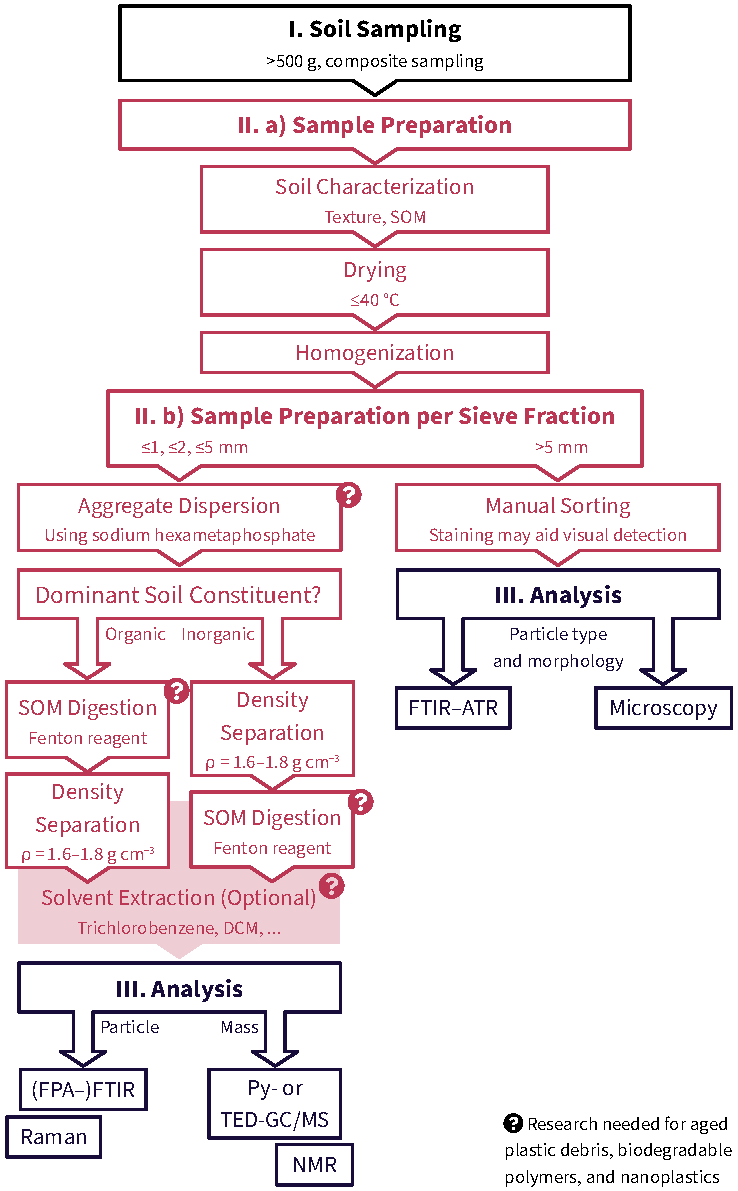
\includegraphics[width=3.28in]{figures/analytical-overview}
	\caption{Suggestions for best-practice sample preparation for microplastic analysis of soil.}
	\label{fig:analytical-overview}
	\forceversofloat
\end{figure}

Sample preparation involves drying below \SI{60}{\degreeCelsius}, ideally \SI{<=40}{\degreeCelsius}, to avoid any deterioration of microplastic particles
(Section~\ref{sec:analytical-techniques:drying}). This may be particularly important for preserving biodegradable polymers. Whether freeze drying might fragment microplastics by frost wedging is unknown to date. After sufficient homogenization, soil should be sieved to \SIlist{1;2;5}{\milli\meter} to comply both with established soil texture classifications and microplastic definitions (Section~\ref{sec:analytical-techniques:homogenization}).
Further sample preparation is performed per sieve fraction. While manual sorting of macroplastics often suffices for the sieve fraction \SI{>5}{\milli\meter}, finer fractions (\SIlist{<=1;<=2;<=5}{\milli\meter}) may require dispersing soil aggregates to retrieve occluded microplastics
(Section~\ref{sec:analytical-techniques:dispersion}). However, it still needs to be assessed whether soil sieving and dispersion methods like agitation with sodium hexametaphosphate solution or ultrasonication may fragment aged or biodegradable microplastics as well as nanoplastics.

If inorganic minerals are dominant in the investigated soil, the microplastic fraction should be preconcentrated by density separation
(Section~\ref{sec:analytical-techniques:density-separation}). Selecting a specific density separation setup involves careful consideration of the targeted polymers and particle sizes, recoveries, cost efficiency, ease of operation, and environmental concerns. To extract all major polymer types, aiming for determination of total plastic contents in soil, high-density solutions ($\rho$ = \SIrange{1.6}{1.8}{\gram\per\cubic\centi\meter})
such as \ch{NaBr} or \ac{spt} are recommended. Solutions with lower densities like saturated \ch{NaCl} solution may be useful for target analyses, particularly of \ac{pe}, \ac{pp}, and \ac{ps}. In any case, separation methods should be validated by recovery experiments that involve spiking known polymer types and particle sizes to a realistic,
well-characterized soil matrix. In addition, potential sources of contamination need to be closely monitored, for instance, by using procedural blanks and closed containers. In this respect, separation funnels may be a promising alternative to open vessels that are currently the most common equipment for microplastic separation.

Additional \ac{som} removal (Section~\ref{sec:analytical-techniques:som-removal}) is necessary if analytical interferences from \ac{som} are expected. Ideally,
\ac{som} removal agents should efficiently digest or degrade \ac{som} while preserving microplastic analytes. Current literature recommends Fenton reagent, which allows for efficient \ac{som} oxidation at controlled temperatures (\SI{<=40}{\degreeCelsius}) and thus has minimal impact on microplastics. An alternative may be selective extraction of polymers in organic solvents like \ac{dcm} or \ac{tcb} at elevated temperature
(Section~\ref{sec:analytical-techniques:solvent-extraction}) while keeping interfering \ac{som}
in the precipitate. By doing so, physical properties of the particles will be lost. Nonetheless, such approaches may become increasingly relevant due to the growing demand for quantitative methods for biodegradable plastics, which are more sensitive to degradation during sample preparation than conventional polymers.

The major options for subsequent microplastic analysis are visual microscopy for particles \SI{>500}{\micro\meter}
(Section~\ref{sec:analytical-techniques:microscopy}), \ac{ftir} or Raman
(micro)spectroscopy for smaller particles
(Section~\ref{sec:analytical-techniques:spectroscopy}), mass-based,
thermoanalytical methods (Section \ref{sec:analytical-techniques:thermoanalysis}), and quantitative \ac{hnmr} spectroscopy (Section~\ref{sec:analytical-techniques:further-techniques}). If particle numbers, sizes, and morphology are of specific interest to the research question, spectroscopic methods are favorable. For quantifying plastic pollution in terms of mass, which has been argued to be more comparable, thermoanalytical methods and \ac{hnmr} spectroscopy may be preferred. The associated \acp{lod} in terms of microplastic size need to be stated, also taking previous sample preparation steps into account.

Terrestrial microplastics research is a quickly evolving field characterized by an extraordinarily high diversity of newly developed or refined analytical approaches. While this challenges future standardization, active method development offers great opportunities for innovations and microplastic analyses tailored to specific research questions. However, harmonization needs to start with uniform communication of microplastic quantities in particles \si{\per\kilo\gram} for microplastic counts and in \si{\micro\gram} or \si{\gram\per\kilo\gram} for mass-based results \citep{BraunMicroplastics2018}. Furthermore, quality control measures should be implemented at an early stage of method development.
This includes
\begin{enumerate*}
	\item controlling contamination by working plastic-free and including blank measurements,
	\item thorough documentation of the studied soil, sample preparation, and analytical methods, and
	\item method validation with recovery tests and an assessment of analytical limitations
\end{enumerate*}.
In this respect, the best practices for terrestrial microplastic analysis still need to be established. Because of the complexity and heterogeneity of soil, soil sample preparation for microplastic analysis must be adapted to the specific properties and composition of the examined soil.
This will not only help to ensure efficient matrix removal while conserving microplastics, it will also advance the field towards a better understanding of processes and interactions of microplastic particles with \ac{som} and other soil constituents.
